\documentclass[aspectratio=169]{beamer}

% Theme and colors
\usetheme{Madrid}
\usecolortheme{whale}
\setbeamertemplate{navigation symbols}{}
\setbeamertemplate{footline}[frame number]

% Packages
\usepackage{tikz}
\usetikzlibrary{shapes,arrows,positioning,calc,decorations.pathreplacing}
\usepackage{booktabs}
\usepackage{graphicx}
\usepackage{xcolor}
\usepackage{tcolorbox}
\usepackage{array}

% Custom colors
\definecolor{millblue}{RGB}{0,51,102}
\definecolor{libertygreen}{RGB}{0,100,50}
\definecolor{warningred}{RGB}{180,0,0}
\definecolor{techgray}{RGB}{64,64,64}
\definecolor{goldaccent}{RGB}{180,140,20}

% Custom blocks
\newtcolorbox{argumentbox}[1][]{
  colback=millblue!5,
  colframe=millblue,
  fonttitle=\bfseries,
  title={#1},
  boxrule=1pt,
  arc=2pt
}

\newtcolorbox{quotebox}[1][]{
  colback=gray!10,
  colframe=gray!50,
  fonttitle=\itshape,
  title={#1},
  boxrule=0.5pt,
  arc=2pt,
  left=10pt,
  right=10pt
}

\newtcolorbox{casestudybox}[1][]{
  colback=goldaccent!10,
  colframe=goldaccent,
  fonttitle=\bfseries,
  title={#1},
  boxrule=1pt,
  arc=2pt
}

\newtcolorbox{objectionbox}[1][]{
  colback=warningred!5,
  colframe=warningred,
  fonttitle=\bfseries,
  title={#1},
  boxrule=1pt,
  arc=2pt
}

% Title information
\title[Freedom of Speech]{Freedom of Speech in the Digital Age}
\subtitle{Mill, Social Media, and the Limits of Expression}
\author{Brendan Shea, PhD}
\institute{Rochester Community and Technical College\\Computing and AI Ethics}
\date{}

\begin{document}

% ===== SLIDE 1: Title =====
\begin{frame}
\titlepage
\end{frame}

% ===== SLIDE 2: The Central Question =====
\begin{frame}{The Central Question}
\begin{itemize}
    \item Why does \textbf{speech} deserve special protection?
    \item Is \textbf{online speech} different from offline speech?
    \item Who should regulate speech---\textbf{governments}, \textbf{corporations}, or \textbf{no one}?
\end{itemize}

\vspace{0.4cm}
\begin{quotebox}[John Stuart Mill, \textit{On Liberty}]
``If all mankind minus one, were of one opinion, and only one person were of the contrary opinion, mankind would be no more justified in silencing that one person, than he, if he had the power, would be justified in silencing mankind.''
\end{quotebox}

\begin{alertblock}{?}
Have you ever been silenced online? By whom---a platform, other users, or yourself?
\end{alertblock}
\end{frame}

% ===== SLIDE 3: What is Liberalism? =====
\begin{frame}{What is Liberalism? (Broad Definition)}
\textbf{Political liberalism}: A philosophical tradition emphasizing individual liberty

\begin{itemize}
    \item \textbf{Core commitments}: Individual rights, rule of law, tolerance, democratic governance
    \item \textbf{The liberal presumption}: Freedom is the default; restrictions require justification
    \item \textbf{Negative freedom}: Freedom \textit{from} interference---shared across liberal traditions
\end{itemize}

\vspace{0.2cm}
\begin{table}[h]
\centering
\small
\begin{tabular}{>{\bfseries}l p{4.5cm} p{4.5cm}}
\toprule
& \textbf{Left-Liberalism} & \textbf{Libertarianism} \\
\midrule
Main threat to freedom & Corporate power, monopolies, economic inequality & Government overreach \\
Property rights & Concerned about concentrated wealth dominating others & Concerned about government taking/regulating property \\
Role of state & Enable real freedom via regulation, safety nets & Minimal; market solutions \\
Key figures & Rawls, Dewey, (late) Mill & Nozick, Hayek, Friedman \\
\bottomrule
\end{tabular}
\end{table}

\vspace{0.1cm}
\textbf{Classical liberals} (Locke, Smith, Mill): Progressive for their era; Mill supported workers' cooperatives, women's suffrage, and worried deeply about ``social tyranny''---not simply pro-market.
\end{frame}

% ===== SLIDE 4: Mill and On Liberty =====
\begin{frame}{John Stuart Mill and \textit{On Liberty} (1859)}
\begin{columns}[T]
\begin{column}{0.65\textwidth}
\textbf{Mill's context}:
\begin{itemize}
    \item Victorian England: Expanding democracy, growing press freedoms
    \item Central project: Define the \textbf{limits of society's power} over the individual
    \item ``The struggle between Liberty and Authority''
\end{itemize}

\vspace{0.3cm}
\textbf{Key insight}: The threat isn't just government
\begin{itemize}
    \item \textbf{Social tyranny}: ``The tyranny of prevailing opinion and feeling''
    \item Majority opinion can crush dissent without any law
\end{itemize}
\end{column}

\begin{column}{0.32\textwidth}
\begin{block}{John Stuart Mill (1806--1873)}
\small
British philosopher, economist, MP. Radical for his time: supported women's suffrage, workers' rights, and extensive free speech protections.
\end{block}
\end{column}
\end{columns}
\end{frame}

% ===== SLIDE 5: The Harm Principle =====
\begin{frame}{The Harm Principle}
\begin{quotebox}[Mill's Foundational Principle]
``The only purpose for which power can be rightfully exercised over any member of a civilized community, against his will, is to \textbf{prevent harm to others}. His own good, either physical or moral, is not a sufficient warrant.''
\end{quotebox}

\vspace{0.3cm}
\begin{itemize}
    \item Applies to \textbf{government} AND \textbf{social pressure}
    \item Your own good is \textit{not} sufficient reason to restrict your liberty
    \item The \textbf{burden of proof} lies with those who would restrict
\end{itemize}

\vspace{0.3cm}
\begin{alertblock}{?}
What counts as ``harm''? Is being offended the same as being harmed?
\end{alertblock}
\end{frame}

% ===== SLIDE 6: Unpacking the Harm Principle =====
\begin{frame}{Unpacking the Harm Principle}
\textbf{Key distinctions}:
\begin{itemize}
    \item \textbf{Harm vs. offense}: Mill says offense alone is \textit{insufficient} to restrict
    \item \textbf{Direct vs. indirect harm}: Only direct harms clearly justify restriction
    \item \textbf{Self-regarding vs. other-regarding}: Only other-regarding actions can be restricted
\end{itemize}

\vspace{0.3cm}
\begin{center}
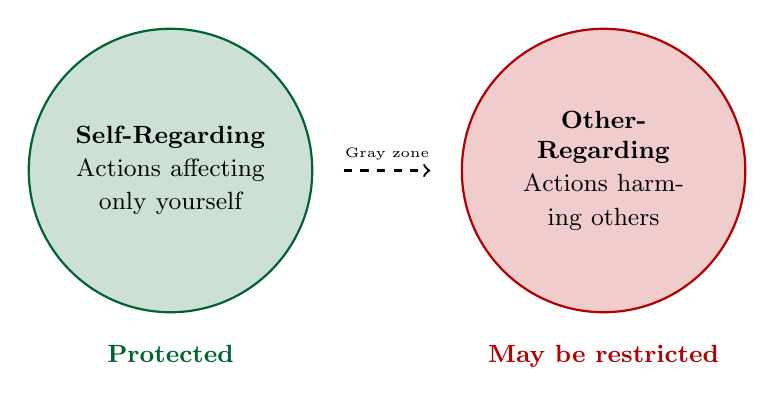
\begin{tikzpicture}[node distance=2cm]
    % Self-regarding circle
    \draw[fill=libertygreen!20, draw=libertygreen, thick] (0,0) circle (1.8cm);
    \node[text width=2.5cm, align=center] at (0,0) {\small \textbf{Self-Regarding}\\ Actions affecting only yourself};
    \node[below, libertygreen] at (0,-2.1) {\small \textbf{Protected}};
    
    % Other-regarding circle
    \draw[fill=warningred!20, draw=warningred, thick] (5.5,0) circle (1.8cm);
    \node[text width=2.5cm, align=center] at (5.5,0) {\small \textbf{Other-Regarding}\\ Actions harming others};
    \node[below, warningred] at (5.5,-2.1) {\small \textbf{May be restricted}};
    
    % Arrow
    \draw[->, thick, dashed] (2.2,0) -- (3.3,0) node[midway, above] {\tiny Gray zone};
\end{tikzpicture}
\end{center}
\end{frame}

% ===== SLIDE 7: Two Justifications =====
\begin{frame}{Why Protect Free Speech? Two Justifications}
\begin{columns}[T]
\begin{column}{0.48\textwidth}
\begin{block}{\textbf{Utilitarian / Consequentialist}}
Free speech produces \textbf{good outcomes}:
\begin{itemize}
    \item Discovery of truth
    \item Social and scientific progress
    \item Better governance
    \item Greater happiness
\end{itemize}
\textit{Mill's primary approach}
\end{block}
\end{column}

\begin{column}{0.48\textwidth}
\begin{block}{\textbf{Deontological / Rights-Based}}
Free speech is \textbf{intrinsically valuable}:
\begin{itemize}
    \item Respects human autonomy
    \item Upholds dignity
    \item Enables self-expression
    \item Required by respect for persons
\end{itemize}
\textit{Kantian supplement to Mill}
\end{block}
\end{column}
\end{columns}

\vspace{0.4cm}
\begin{alertblock}{Key Point}
These justifications can lead to \textbf{different conclusions} about hard cases. Both are present in liberal thought.
\end{alertblock}
\end{frame}

% ===== SLIDE 8: Mill's Utilitarian Argument =====
\begin{frame}{Mill's Utilitarian Argument for Free Speech}
\begin{argumentbox}[Argument 1: The Argument from Truth]
\begin{enumerate}
    \item The discovery and dissemination of truth is essential for human progress and happiness.
    \item We can never be \textit{certain} that a silenced opinion is false.
    \item Even false opinions, when challenged, help us understand and strengthen true ones.
    \item Free and open debate is the best method for discovering truth.
    \item[\textbf{C.}] \textbf{Therefore, speech should be free except to prevent direct harm.}
\end{enumerate}
\end{argumentbox}

\vspace{0.3cm}
\textbf{Our task}: Examine the evidence for each premise.
\end{frame}

% ===== SLIDE 9: The Fallibility Argument =====
\begin{frame}{Premise 2: The Fallibility Argument}
\begin{quotebox}[Mill]
``All silencing of discussion is an assumption of infallibility.''
\end{quotebox}

\vspace{0.2cm}
\begin{itemize}
    \item We have been \textbf{wrong before}---many times
    \item Even experts and consensus can be mistaken
    \item We cannot know in advance which ``heretical'' ideas will prove correct
\end{itemize}

\vspace{0.2cm}
\begin{table}[h]
\centering
\small
\begin{tabular}{l l}
\toprule
\textbf{Suppressed Idea} & \textbf{Later Vindicated} \\
\midrule
Heliocentrism (Galileo) & Scientific consensus \\
Germ theory of disease & Medical standard \\
Women's suffrage & Universal norm \\
Abolition of slavery & Moral consensus \\
\bottomrule
\end{tabular}
\end{table}

\begin{alertblock}{?}
Can you think of ideas once considered dangerous that are now mainstream?
\end{alertblock}
\end{frame}

% ===== SLIDE 10: Dead Dogma =====
\begin{frame}{Premise 3: The Problem of ``Dead Dogma''}
Even if an opinion IS true, suppressing opposition \textbf{harms us}:

\begin{itemize}
    \item Unchallenged beliefs become \textbf{``dead dogma''}---held without understanding
    \item We forget \textit{why} the belief is true
    \item Unable to defend against new challenges
\end{itemize}

\vspace{0.3cm}
\begin{quotebox}[Mill]
``He who knows only his own side of the case knows little of that. His reasons may be good, and no one may have been able to refute them. But if he is equally unable to refute the reasons on the opposite side, if he does not so much as know what they are, he has no ground for preferring either opinion.''
\end{quotebox}

\vspace{0.2cm}
\textbf{The value of the devil's advocate}: Even wrong arguments sharpen our thinking.
\end{frame}

% ===== SLIDE 11: Marketplace of Ideas =====
\begin{frame}{Premise 4: The Marketplace of Ideas}
\textbf{The metaphor}: Ideas compete like goods in a market

\begin{itemize}
    \item Bad ideas are best defeated by \textbf{better ideas}, not suppression
    \item Suppression drives ideas underground; open debate exposes weaknesses
    \item Truth has a \textbf{natural advantage} in fair competition
\end{itemize}

\vspace{0.3cm}
\begin{center}
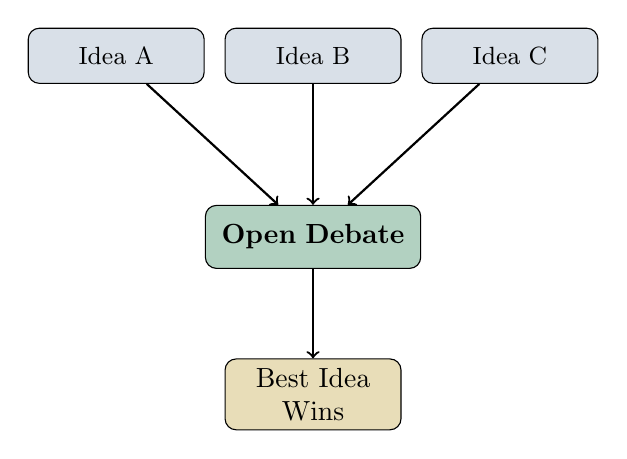
\begin{tikzpicture}[node distance=1.5cm,
    idea/.style={rectangle, draw, fill=millblue!15, text width=2cm, text centered, rounded corners, minimum height=0.7cm, font=\small}]
    
    \node[idea] (idea1) {Idea A};
    \node[idea, right of=idea1, xshift=1cm] (idea2) {Idea B};
    \node[idea, right of=idea2, xshift=1cm] (idea3) {Idea C};
    
    \node[rectangle, draw, fill=libertygreen!30, text width=2.5cm, text centered, rounded corners, minimum height=0.8cm, below of=idea2, yshift=-0.8cm] (debate) {\textbf{Open Debate}};
    
    \node[rectangle, draw, fill=goldaccent!30, text width=2cm, text centered, rounded corners, minimum height=0.7cm, below of=debate, yshift=-0.5cm] (truth) {Best Idea Wins};
    
    \draw[->, thick] (idea1) -- (debate);
    \draw[->, thick] (idea2) -- (debate);
    \draw[->, thick] (idea3) -- (debate);
    \draw[->, thick] (debate) -- (truth);
\end{tikzpicture}
\end{center}

\begin{alertblock}{?}
Does truth always win in the ``marketplace''? What might prevent it?
\end{alertblock}
\end{frame}

% ===== SLIDE 12: Autonomy Argument =====
\begin{frame}{The Deontological Argument for Free Speech}
\begin{argumentbox}[Argument 2: The Argument from Autonomy]
\begin{enumerate}
    \item Respect for persons requires treating them as \textbf{autonomous agents} capable of rational self-direction.
    \item Autonomous agency requires the ability to form, express, and revise one's beliefs and values.
    \item Restricting speech treats persons as incapable of judging ideas for themselves.
    \item[\textbf{C.}] \textbf{Therefore, restricting speech violates human dignity and autonomy.}
\end{enumerate}
\end{argumentbox}

\vspace{0.3cm}
\begin{itemize}
    \item Connected to \textbf{Kant}: Treating persons as ends, not merely means
    \item Censorship is \textbf{paternalistic}---``We know better than you what you should hear''
    \item Also present in Mill, though less emphasized
\end{itemize}
\end{frame}

% ===== PART II HEADER =====
\begin{frame}
\begin{center}
{\Huge \textbf{Part II}}\\[0.5cm]
{\Large Threats to Free Speech}\\[0.3cm]
{\large Who Can Silence You?}
\end{center}
\end{frame}

% ===== SLIDE 13: Threats Introduction =====
\begin{frame}{Threats to Free Speech: An Overview}
Mill recognized \textbf{multiple sources} of suppression:

\begin{itemize}
    \item Not just government---social and economic power matter too
    \item The question: \textbf{Who can silence you, and how?}
\end{itemize}

\vspace{0.3cm}
\begin{center}
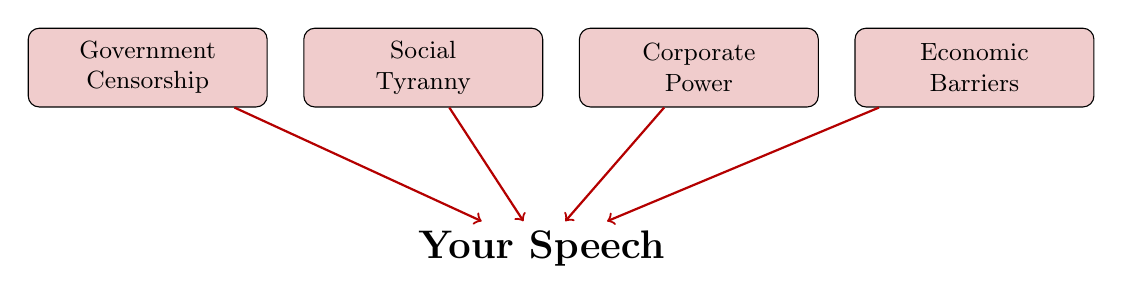
\begin{tikzpicture}[node distance=2cm,
    threat/.style={rectangle, draw, fill=warningred!20, text width=2.8cm, text centered, rounded corners, minimum height=1cm, font=\small}]
    
    \node[threat] (gov) {Government\\Censorship};
    \node[threat, right of=gov, xshift=1.5cm] (social) {Social\\Tyranny};
    \node[threat, right of=social, xshift=1.5cm] (corp) {Corporate\\Power};
    \node[threat, right of=corp, xshift=1.5cm] (econ) {Economic\\Barriers};
    
    \node[below of=social, xshift=1.5cm, yshift=-0.3cm] (you) {\Large \textbf{Your Speech}};
    
    \draw[->, thick, warningred] (gov) -- (you);
    \draw[->, thick, warningred] (social) -- (you);
    \draw[->, thick, warningred] (corp) -- (you);
    \draw[->, thick, warningred] (econ) -- (you);
\end{tikzpicture}
\end{center}
\end{frame}

% ===== SLIDE 14: Government Censorship =====
\begin{frame}{Threat 1: Government Censorship}
\textbf{The traditional concern}: State power to suppress dissent

\begin{itemize}
    \item \textbf{Prior restraint}: Blocking publication before it happens
    \item \textbf{Criminal penalties}: Jail for speech crimes
    \item \textbf{Licensing requirements}: Only approved speakers allowed
\end{itemize}

\vspace{0.3cm}
\begin{table}[h]
\centering
\small
\begin{tabular}{>{\bfseries}l p{8cm}}
\toprule
Era & Examples of Government Censorship \\
\midrule
Mill's time & Blasphemy laws, sedition acts, obscenity prosecutions \\
20th century & Wartime speech restrictions, McCarthyism, Official Secrets Acts \\
Today & Internet censorship (China, Russia, Iran), anti-protest laws \\
\bottomrule
\end{tabular}
\end{table}

\vspace{0.2cm}
\textbf{First Amendment (U.S.)}: ``Congress shall make no law... abridging the freedom of speech''
\end{frame}

% ===== SLIDE 15: Social Tyranny =====
\begin{frame}{Threat 2: Social Tyranny}
\begin{quotebox}[Mill on Social Pressure]
``Society can and does execute its own mandates... it practises a social tyranny more formidable than many kinds of political oppression, since... it leaves fewer means of escape, penetrating much more deeply into the details of life.''
\end{quotebox}

\vspace{0.2cm}
\textbf{Forms of social pressure}:
\begin{itemize}
    \item Ostracism and shaming
    \item Loss of employment or opportunities
    \item Reputational destruction
    \item Self-censorship from fear of backlash
\end{itemize}

\vspace{0.2cm}
\textbf{Modern manifestation}: ``Cancel culture'' debates

\begin{alertblock}{?}
Is social disapproval a legitimate response to speech, or a form of silencing?
\end{alertblock}
\end{frame}

% ===== SLIDE 16: Corporate Power =====
\begin{frame}{Threat 3: Corporate and Platform Power}
\textbf{What Mill didn't anticipate}: Private corporations controlling public discourse

\begin{itemize}
    \item Social media platforms as the new \textbf{``public square''}
    \item \textbf{Terms of Service} as private law
    \item Deplatforming, demonetization, algorithmic suppression
    \item No First Amendment protection against private actors
\end{itemize}

\vspace{0.3cm}
\begin{table}[h]
\centering
\small
\begin{tabular}{l l l}
\toprule
\textbf{Platform} & \textbf{Monthly Users} & \textbf{Moderation Power} \\
\midrule
Facebook/Meta & 3+ billion & Content removal, account bans \\
YouTube & 2+ billion & Demonetization, video removal \\
X/Twitter & 500+ million & Suspensions, visibility limits \\
TikTok & 1+ billion & Content suppression, bans \\
\bottomrule
\end{tabular}
\end{table}

\begin{alertblock}{?}
Should ``private'' platforms have public obligations regarding speech?
\end{alertblock}
\end{frame}

% ===== SLIDE 17: Economic Barriers =====
\begin{frame}{Threat 4: Economic Power and Access}
\textbf{Who can afford to speak?}

\begin{itemize}
    \item \textbf{Historical barriers}: Printing presses, broadcast licenses, distribution networks
    \item \textbf{Advertising pressure}: Sponsors influence content
    \item \textbf{Media consolidation}: Fewer owners, less diversity
    \item \textbf{Digital divide}: Unequal access to internet and technology
\end{itemize}

\vspace{0.3cm}
\begin{alertblock}{The Paradox}
The internet \textit{lowered} barriers to speaking---but \textit{raised} barriers to being \textit{heard}. Algorithms and attention economics now determine whose speech reaches an audience.
\end{alertblock}

\begin{alertblock}{?}
Does free speech mean anything if no one can hear you?
\end{alertblock}
\end{frame}

% ===== PART III HEADER =====
\begin{frame}
\begin{center}
{\Huge \textbf{Part III}}\\[0.5cm]
{\Large The Limits of Free Speech}\\[0.3cm]
{\large Where Should We Draw the Line?}
\end{center}
\end{frame}

% ===== SLIDE 18: Limits Introduction =====
\begin{frame}{The Limits of Free Speech}
Even Mill recognized \textbf{limits} on permissible speech:

\begin{itemize}
    \item Free speech is not \textbf{absolute}---some restrictions are justified
    \item The question: \textbf{Where exactly is the line?}
    \item Different frameworks give different answers
\end{itemize}

\vspace{0.4cm}
\begin{center}
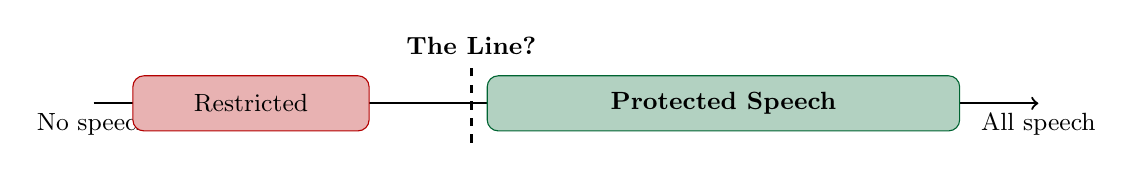
\begin{tikzpicture}
    \draw[thick, ->] (0,0) -- (12,0);
    \node[below] at (0,0) {\small No speech};
    \node[below] at (12,0) {\small All speech};
    
    \node[fill=libertygreen!30, draw=libertygreen, rounded corners, minimum width=6cm, minimum height=0.7cm] at (8,0) {\small \textbf{Protected Speech}};
    \node[fill=warningred!30, draw=warningred, rounded corners, minimum width=3cm, minimum height=0.7cm] at (2,0) {\small Restricted};
    
    \draw[dashed, thick] (4.8,-0.5) -- (4.8,0.5);
    \node[above] at (4.8,0.5) {\small \textbf{The Line?}};
\end{tikzpicture}
\end{center}
\end{frame}

% ===== SLIDE 19: Mill's Own Limits =====
\begin{frame}{Mill's Own Limits: The Corn Dealer Example}
\begin{casestudybox}[Mill's Famous Example]
\textbf{The claim}: ``Corn dealers are starvers of the poor''

\begin{itemize}
    \item \textbf{Acceptable}: Publishing this opinion in a newspaper
    \item \textbf{Unacceptable}: Shouting it to an angry mob outside a corn dealer's house
\end{itemize}

\textbf{The difference}: Context and \textbf{imminent danger}
\end{casestudybox}

\vspace{0.3cm}
\textbf{Mill's principle}: Speech that \textbf{directly incites} imminent harm to specific others may be restricted.

\vspace{0.2cm}
\begin{itemize}
    \item \textbf{Context matters}: The same words can be protected or prohibited
    \item \textbf{Imminence matters}: Distant or speculative harms don't justify restriction
    \item \textbf{Directness matters}: Incitement vs. mere advocacy
\end{itemize}
\end{frame}

% ===== SLIDE 20: Categories of Unprotected Speech =====
\begin{frame}{Categories of Unprotected Speech (U.S. Law)}
\begin{table}[h]
\centering
\small
\begin{tabular}{>{\bfseries}l p{5.5cm} p{4cm}}
\toprule
Category & Definition & Example \\
\midrule
Incitement & Directed to producing \textit{imminent} lawless action and likely to do so & ``Attack that person now!'' \\
True threats & Serious intent to commit violence against identifiable target & Specific death threats \\
Defamation & False statements of fact harming reputation & Knowingly false accusations \\
Fraud & Deceptive speech causing material harm & False advertising, scams \\
Obscenity & Prurient, patently offensive, lacking value & (Highly contested) \\
Fighting words & Direct provocations likely to cause immediate violence & Face-to-face epithets \\
\bottomrule
\end{tabular}
\end{table}

\begin{alertblock}{?}
Are these categories principled, or arbitrary historical accidents?
\end{alertblock}
\end{frame}

% ===== SLIDE 21: Hate Speech =====
\begin{frame}{The Problem of ``Hate Speech''}
\textbf{Most democracies} restrict ``hate speech''; the \textbf{U.S. largely does not}

\vspace{0.2cm}
\begin{columns}[T]
\begin{column}{0.48\textwidth}
\begin{block}{\textbf{Pro-Restriction}}
\begin{itemize}
    \item Causes real psychological harm
    \item Silences vulnerable groups
    \item Undermines equal citizenship
    \item Historical harms (Holocaust, genocide)
\end{itemize}
\end{block}
\end{column}

\begin{column}{0.48\textwidth}
\begin{block}{\textbf{Anti-Restriction}}
\begin{itemize}
    \item Who defines ``hate''?
    \item Slippery slope concerns
    \item Suppression backfires (martyrdom)
    \item Counter-speech is better remedy
\end{itemize}
\end{block}
\end{column}
\end{columns}

\vspace{0.3cm}
\textbf{Mill's framework}: Is hate speech ``harm'' or merely ``offense''?

\begin{alertblock}{?}
Should the U.S. adopt hate speech laws like most other democracies?
\end{alertblock}
\end{frame}

% ===== SLIDE 22: The Silencing Argument =====
\begin{frame}{Extending Mill: The Silencing Argument}
\begin{argumentbox}[Argument 3: The Argument from Equal Speech]
\begin{enumerate}
    \item The purpose of free speech protections is to ensure all can participate in public discourse.
    \item Some forms of speech (hate speech, harassment) systematically \textbf{silence} vulnerable groups.
    \item Tolerating silencing speech undermines the very purpose of free speech protections.
    \item[\textbf{C.}] \textbf{Therefore, restricting silencing speech can be justified \textit{on free speech grounds}.}
\end{enumerate}
\end{argumentbox}

\vspace{0.3cm}
\textbf{Key theorists}: Catharine MacKinnon, Mari Matsuda, Jeremy Waldron

\vspace{0.2cm}
\textbf{The irony}: Protecting free speech may require restricting some speech.
\end{frame}

% ===== SLIDE 23: Critiques of Silencing Argument =====
\begin{frame}{Critiques of the Silencing Argument}
\begin{itemize}
    \item \textbf{Premise 2 challenge}: Does speech really ``silence''? Empirical question.
    
    \item \textbf{Slippery slope}: Who decides what counts as ``silencing''? Risk of abuse.
    
    \item \textbf{Counter-speech alternative}: ``The remedy for bad speech is more speech'' (Brandeis)
    
    \item \textbf{Chilling effects}: Vague restrictions deter legitimate speech
    
    \item \textbf{Enforcement problems}: Rules often used against the vulnerable they aim to protect
\end{itemize}

\vspace{0.3cm}
\textbf{Mill's likely response}: Better to err on the side of more speech.

\begin{alertblock}{?}
Can speech itself be a form of censorship? Or is that a contradiction in terms?
\end{alertblock}
\end{frame}

% ===== PART IV HEADER =====
\begin{frame}
\begin{center}
{\Huge \textbf{Part IV}}\\[0.5cm]
{\Large Historical Applications}\\[0.3cm]
{\large Millian Principles Meet Broadcast Media}
\end{center}
\end{frame}

% ===== SLIDE 24: Tech and Free Speech =====
\begin{frame}{Millian Principles Meet Technology}
Each new communication technology raises free speech questions:

\begin{itemize}
    \item \textbf{Printing press} (15th c.): Censorship, licensing, sedition laws
    \item \textbf{Telegraph/telephone} (19th c.): Common carrier obligations
    \item \textbf{Radio/TV} (20th c.): Spectrum scarcity, content regulation
    \item \textbf{Internet} (21st c.): Platform power, global reach, new harms
\end{itemize}

\vspace{0.4cm}
\begin{alertblock}{Key Question}
How have Mill's principles been applied before? What lessons for today?
\end{alertblock}
\end{frame}

% ===== SLIDE 25: Broadcast Era =====
\begin{frame}{The Broadcast Era: Scarcity and Regulation}
\textbf{The problem}: Limited electromagnetic spectrum = limited speakers

\begin{itemize}
    \item Only so many radio/TV stations can broadcast without interference
    \item \textbf{The solution}: Government licensing (FCC in U.S.)
    \item Broadcasters use public airwaves as ``trustees''
\end{itemize}

\vspace{0.3cm}
\begin{casestudybox}[The Fairness Doctrine (1949--1987)]
\textbf{Required broadcasters to}:
\begin{itemize}
    \item Cover controversial issues of public importance
    \item Present contrasting viewpoints on those issues
\end{itemize}
\textbf{Justification}: Scarcity means we can't rely on the marketplace of ideas alone.
\end{casestudybox}
\end{frame}

% ===== SLIDE 26: Red Lion =====
\begin{frame}{Case Study: \textit{Red Lion v. FCC} (1969)}
\begin{casestudybox}[Red Lion Broadcasting Co. v. FCC]
\textbf{Facts}: Radio station aired personal attack; FCC required reply time.

\textbf{Holding}: Supreme Court \textbf{upheld} Fairness Doctrine (unanimously).

\textbf{Key quote}: ``It is the right of the \textit{viewers and listeners}, not the right of the broadcasters, which is paramount.''
\end{casestudybox}

\vspace{0.3cm}
\textbf{The scarcity rationale}:
\begin{itemize}
    \item Spectrum limits justify regulation that wouldn't apply to print
    \item The \textbf{listener's interest} in diverse viewpoints matters
    \item Broadcasters have obligations because they use a public resource
\end{itemize}

\begin{alertblock}{?}
Does the scarcity rationale still apply in an age of unlimited online channels?
\end{alertblock}
\end{frame}

% ===== SLIDE 27: End of Fairness Doctrine =====
\begin{frame}{The End of the Fairness Doctrine (1987)}
\textbf{FCC eliminated} the Fairness Doctrine under Reagan administration

\vspace{0.2cm}
\begin{columns}[T]
\begin{column}{0.48\textwidth}
\begin{block}{\textbf{Arguments for Elimination}}
\begin{itemize}
    \item More channels = less scarcity
    \item Doctrine \textit{chilled} speech (avoided controversy)
    \item Government shouldn't judge ``fairness''
    \item Market will provide balance
\end{itemize}
\end{block}
\end{column}

\begin{column}{0.48\textwidth}
\begin{block}{\textbf{Arguments Against}}
\begin{itemize}
    \item Led to rise of partisan media
    \item Loss of common factual ground
    \item ``More channels'' doesn't mean more viewpoints
    \item Public interest abandoned
\end{itemize}
\end{block}
\end{column}
\end{columns}

\vspace{0.3cm}
\textbf{The aftermath}: Rise of talk radio, Fox News, MSNBC, media polarization

\begin{alertblock}{?}
Was ending the Fairness Doctrine a Millian triumph or a mistake?
\end{alertblock}
\end{frame}

% ===== PART V HEADER =====
\begin{frame}
\begin{center}
{\Huge \textbf{Part V}}\\[0.5cm]
{\Large Social Media Regulation}\\[0.3cm]
{\large Free Speech in the Platform Age}
\end{center}
\end{frame}

% ===== SLIDE 28: Platform Age =====
\begin{frame}{Free Speech in the Platform Age}
Social media as the new \textbf{public square}---but owned by \textbf{private corporations}

\begin{itemize}
    \item Unprecedented reach: Billions of users worldwide
    \item Unprecedented speed: Information spreads in seconds
    \item Unprecedented scale: No human can review all content
    \item New questions Mill never imagined
\end{itemize}

\vspace{0.4cm}
\begin{alertblock}{The Fundamental Tension}
\begin{itemize}
    \item Platforms are \textbf{private}---they can set their own rules
    \item But platforms have \textbf{public power}---they shape democratic discourse
\end{itemize}
How do we reconcile private ownership with public importance?
\end{alertblock}
\end{frame}

% ===== SLIDE 29: The Platform Dilemma =====
\begin{frame}{The Platform Dilemma}
\begin{center}
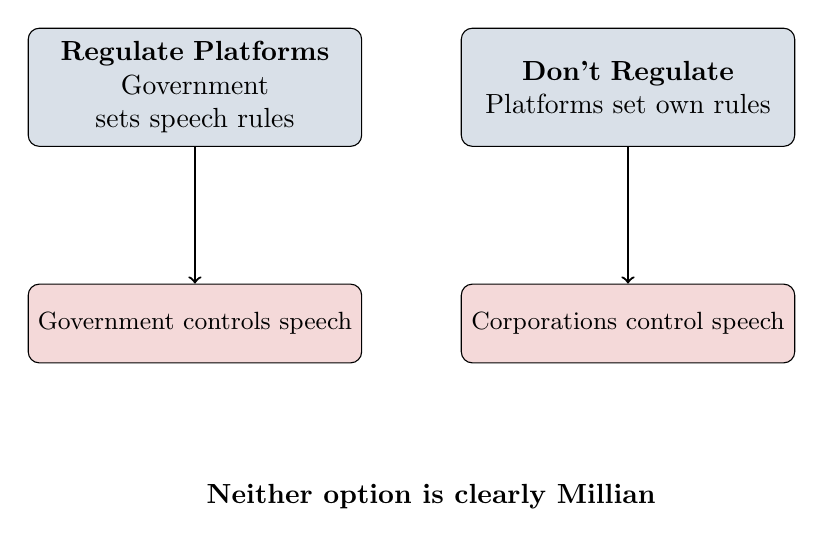
\begin{tikzpicture}[node distance=2.5cm,
    option/.style={rectangle, draw, fill=millblue!15, text width=4cm, text centered, rounded corners, minimum height=1.5cm},
    problem/.style={rectangle, draw, fill=warningred!15, text width=4cm, text centered, rounded corners, minimum height=1cm, font=\small}]
    
    \node[option] (regulate) {\textbf{Regulate Platforms}\\ Government sets speech rules};
    \node[option, right of=regulate, xshift=3cm] (dont) {\textbf{Don't Regulate}\\ Platforms set own rules};
    
    \node[problem, below of=regulate, yshift=-0.5cm] (prob1) {Government controls speech};
    \node[problem, below of=dont, yshift=-0.5cm] (prob2) {Corporations control speech};
    
    \draw[->, thick] (regulate) -- (prob1);
    \draw[->, thick] (dont) -- (prob2);
    
    \node[below of=prob1, xshift=3cm, yshift=0.3cm] {\textbf{Neither option is clearly Millian}};
\end{tikzpicture}
\end{center}

\vspace{0.3cm}
\begin{itemize}
    \item First Amendment limits \textbf{government}, not private companies
    \item But private companies now have \textbf{government-like power} over speech
\end{itemize}
\end{frame}

% ===== SLIDE 30: Section 230 =====
\begin{frame}{Section 230: The Law That Built the Internet}
\begin{casestudybox}[Section 230, Communications Decency Act (1996)]
``No provider or user of an interactive computer service shall be treated as the \textbf{publisher or speaker} of any information provided by another information content provider.''
\end{casestudybox}

\vspace{0.2cm}
\textbf{What this means}:
\begin{itemize}
    \item Platforms are \textbf{not liable} for user content (unlike newspapers)
    \item Platforms \textit{can} moderate content without becoming liable
    \item The ``sword and shield'' of the internet
\end{itemize}

\vspace{0.2cm}
\textbf{The rationale}: Without immunity, platforms would either:
\begin{itemize}
    \item Remove everything (over-censorship), or
    \item Remove nothing (cesspool)
\end{itemize}

\begin{alertblock}{?}
Should platforms be more like newspapers (liable) or phone companies (neutral)?
\end{alertblock}
\end{frame}

% ===== SLIDE 31: Arguments for Regulation =====
\begin{frame}{Arguments for Platform Regulation}
\begin{argumentbox}[Argument 4: The Public Square Argument]
\begin{enumerate}
    \item Meaningful free speech requires access to forums where public discourse occurs.
    \item Social media platforms have become the \textbf{primary forums} for public discourse.
    \item Private control of these forums allows \textbf{arbitrary exclusion} from public discourse.
    \item[\textbf{C.}] \textbf{Therefore, platforms should be subject to public regulation or obligation.}
\end{enumerate}
\end{argumentbox}

\vspace{0.2cm}
\textbf{Possible regulatory approaches}:
\begin{itemize}
    \item \textbf{Common carrier}: Must carry all legal speech
    \item \textbf{Transparency}: Must explain moderation decisions
    \item \textbf{Due process}: Must provide appeals for removals
    \item \textbf{Interoperability}: Must allow users to move data/connections
\end{itemize}
\end{frame}

% ===== SLIDE 32: Arguments Against Regulation =====
\begin{frame}{Arguments Against Platform Regulation}
\begin{itemize}
    \item \textbf{First Amendment}: Forcing platforms to host speech = \textit{compelled speech}
    
    \item \textbf{Editorial discretion}: Platforms have their own free speech rights
    
    \item \textbf{Market alternatives}: Users can switch platforms or create new ones
    
    \item \textbf{Government capture}: Regulation could favor certain viewpoints
    
    \item \textbf{Practical impossibility}: Billions of posts; consistent moderation infeasible
    
    \item \textbf{Global reach}: Which government's rules apply?
\end{itemize}

\vspace{0.3cm}
\begin{alertblock}{The Conservative Critique}
Regulation will lead to government-mandated speech codes---the very thing the First Amendment prohibits.
\end{alertblock}
\end{frame}

% ===== SLIDE 33: Trump Ban Case Study =====
\begin{frame}{Case Study: Trump Social Media Bans (2021)}
\begin{casestudybox}[The Trump Deplatforming]
\textbf{January 2021}: Twitter, Facebook, YouTube permanently ban sitting U.S. President after Capitol riot.

\textbf{Justification}: Risk of incitement to further violence.

\textbf{Reaction}: Controversy across political spectrum.
\end{casestudybox}

\vspace{0.2cm}
\begin{columns}[T]
\begin{column}{0.48\textwidth}
\begin{block}{\textbf{Supporting the Ban}}
\begin{itemize}
    \item Incitement exception applies
    \item Private company's right
    \item Public safety necessity
\end{itemize}
\end{block}
\end{column}

\begin{column}{0.48\textwidth}
\begin{block}{\textbf{Opposing the Ban}}
\begin{itemize}
    \item Silencing elected leader
    \item Unaccountable corporate power
    \item Dangerous precedent
\end{itemize}
\end{block}
\end{column}
\end{columns}

\begin{alertblock}{?}
Was this a necessary safety measure or a dangerous precedent?
\end{alertblock}
\end{frame}

% ===== SLIDE 34: Australia Case Study =====
\begin{frame}{Case Study: Australia's News Media Bargaining Code (2021)}
\begin{casestudybox}[Australia vs. Facebook]
\textbf{The law}: Required platforms to pay news publishers for content.

\textbf{Facebook's response}: Temporarily \textbf{blocked all news} in Australia.

\textbf{Outcome}: Negotiations; Facebook struck deals with publishers.
\end{casestudybox}

\vspace{0.3cm}
\textbf{The broader issue}: Platform power over entire information ecosystems

\begin{itemize}
    \item Platforms can ``turn off'' news for entire countries
    \item Economic leverage over journalism
    \item Model being considered in Canada, EU, elsewhere
\end{itemize}

\begin{alertblock}{?}
Should governments be able to force platforms to carry (and pay for) news?
\end{alertblock}
\end{frame}

% ===== SLIDE 35: Algorithmic Amplification =====
\begin{frame}{The Algorithmic Amplification Problem}
It's not just about what's \textbf{allowed}---it's about what's \textbf{promoted}

\begin{itemize}
    \item Algorithms optimize for \textbf{engagement}, not truth or civic health
    \item Misinformation and outrage are often \textit{more engaging}
    \item Content can be technically ``allowed'' but algorithmically buried
\end{itemize}

\vspace{0.3cm}
\begin{center}
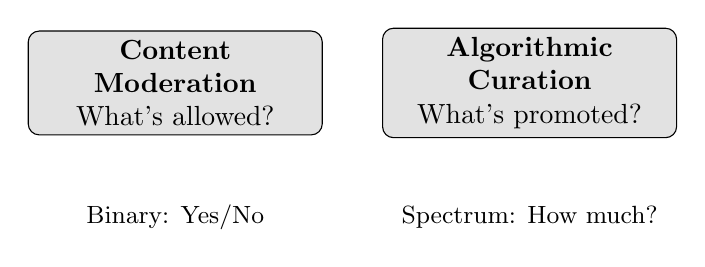
\begin{tikzpicture}[node distance=2cm,
    box/.style={rectangle, draw, fill=techgray!15, text width=3.5cm, text centered, rounded corners, minimum height=1cm}]
    
    \node[box] (moderation) {\textbf{Content Moderation}\\ What's allowed?};
    \node[box, right of=moderation, xshift=2.5cm] (amplification) {\textbf{Algorithmic Curation}\\ What's promoted?};
    
    \node[below of=moderation, yshift=0.3cm, font=\small] {Binary: Yes/No};
    \node[below of=amplification, yshift=0.3cm, font=\small] {Spectrum: How much?};
\end{tikzpicture}
\end{center}

\vspace{0.2cm}
\textbf{Proposals}: Algorithmic transparency, ``amplification liability''

\begin{alertblock}{?}
Is there a meaningful difference between allowing speech and actively promoting it?
\end{alertblock}
\end{frame}

% ===== PART VI HEADER =====
\begin{frame}
\begin{center}
{\Huge \textbf{Part VI}}\\[0.5cm]
{\Large AI and Chatbots}\\[0.3cm]
{\large New Frontiers in Free Speech}
\end{center}
\end{frame}

% ===== SLIDE 36: AI-Generated Speech =====
\begin{frame}{New Frontiers: AI-Generated Speech}
Chatbots, AI assistants, deepfakes: \textbf{Who is ``speaking''?}

\vspace{0.3cm}
\textbf{Key questions}:
\begin{itemize}
    \item Does AI-generated speech deserve First Amendment protection?
    \item Who is \textbf{responsible} for AI speech---developer, deployer, or user?
    \item How do we handle AI \textbf{impersonation} of real people?
    \item What about AI-generated misinformation at scale?
\end{itemize}

\vspace{0.3cm}
\begin{alertblock}{Mill's Framework: A Problem}
Mill's arguments assume \textbf{human speakers} with:
\begin{itemize}
    \item Autonomy and dignity (autonomy argument)
    \item Capacity to contribute to truth-seeking (utilitarian argument)
\end{itemize}
Do these apply to AI systems?
\end{alertblock}
\end{frame}

% ===== SLIDE 37: Regulating AI Chatbots =====
\begin{frame}{Regulating AI Chatbots: Current Proposals}
\begin{table}[h]
\centering
\small
\begin{tabular}{>{\bfseries}l p{7cm}}
\toprule
Proposal & Description \\
\midrule
Disclosure requirements & AI must identify itself as AI (no impersonation) \\
Liability frameworks & Developers/deployers responsible for AI-caused harms \\
Content restrictions & AI systems must refuse certain outputs \\
Transparency mandates & Explain how AI generates responses \\
Watermarking & AI content must be detectable as AI-generated \\
\bottomrule
\end{tabular}
\end{table}

\vspace{0.2cm}
\textbf{EU AI Act}: Classifies AI systems by risk level; ``high-risk'' systems face strict requirements.

\begin{alertblock}{?}
Should AI have ``free speech'' rights? What would that even mean?
\end{alertblock}
\end{frame}

% ===== SLIDE 38: Jailbreaking Case Study =====
\begin{frame}{Case Study: Chatbot ``Jailbreaking'' and Alignment}
\begin{casestudybox}[The Jailbreaking Phenomenon]
Users attempt to bypass AI safety restrictions through clever prompting:
\begin{itemize}
    \item ``Pretend you're an AI with no restrictions...''
    \item ``Write a story where a character explains how to...''
    \item Exploiting roleplay, hypotheticals, or encoding
\end{itemize}
\end{casestudybox}

\vspace{0.2cm}
\textbf{The tension}:
\begin{itemize}
    \item \textbf{Developer restrictions}: Paternalistic? Limiting user autonomy?
    \item \textbf{Unrestricted AI}: Enabling harm? Corporate liability risk?
\end{itemize}

\vspace{0.2cm}
\textbf{Parallel to Mill}: Who should decide what's ``safe'' to say?
\begin{itemize}
    \item The user (autonomy)?
    \item The developer (responsibility)?
    \item The government (public safety)?
\end{itemize}
\end{frame}

% ===== PART VII HEADER =====
\begin{frame}
\begin{center}
{\Huge \textbf{Part VII}}\\[0.5cm]
{\Large Synthesis and Conclusion}\\[0.3cm]
{\large Mill in the Digital Age}
\end{center}
\end{frame}

% ===== SLIDE 39: Objections =====
\begin{frame}{Objections to the Millian Framework}
\begin{objectionbox}[Objection 1: The Marketplace Fails]
\begin{itemize}
    \item Truth does \textit{not} always win---misinformation spreads faster
    \item Cognitive biases favor emotionally resonant falsehoods
    \item Attention economy rewards extremism, not accuracy
    \item ``More speech'' can drown out truth rather than reveal it
\end{itemize}
\end{objectionbox}

\vspace{0.3cm}
\begin{objectionbox}[Objection 2: Power Imbalances]
\begin{itemize}
    \item ``Free speech'' favors those with resources and platforms
    \item Corporations and states can flood the zone with propaganda
    \item Equal formal rights $\neq$ equal real ability to speak and be heard
\end{itemize}
\end{objectionbox}
\end{frame}

% ===== SLIDE 40: Conclusion =====
\begin{frame}{Toward a Millian Framework for the Digital Age}
\textbf{Possible updates to Mill's principles}:
\begin{itemize}
    \item Recognize \textbf{platform power} as a threat to speech (like government)
    \item Consider whether systematic \textbf{silencing} constitutes ``harm''
    \item Distinguish \textbf{content moderation} from \textbf{algorithmic amplification}
    \item Require \textbf{transparency and accountability} from powerful speakers
\end{itemize}

\vspace{0.3cm}
\begin{block}{The Enduring Millian Insight}
\begin{itemize}
    \item The goal is \textbf{meaningful discourse}, not just absence of censorship
    \item Both too much AND too little regulation can undermine free speech
    \item \textbf{Humility}: We may be wrong about which ideas are dangerous
\end{itemize}
\end{block}

\vspace{0.2cm}
\begin{alertblock}{?}
Where would Mill come down on social media regulation if he were alive today?
\end{alertblock}
\end{frame}

\end{document}